\begin{samplecase}
{\bf Fission cross sections: n + ${}^{232}$Th: WKB approach}\newline
It is well known that a systematic approach for fission is difficult to achieve.
It is possible to obtain
very satisfactory fits to fission data with TALYS, but at the expense of using
many adjustable input parameters.
We are performing extensive model calculations to bring somewhat more structure
in the collection of fitting parameters. In the meantime, we include here a
sample case for the description of the fission cross section of $^{232}$Th.
This sample case shows the
WKB approximation to calculate fission transmission coefficients as outlined in
Ref. \cite{Sin2006} and Ref. \cite{Goriely08}. It can be invoked
with the keyword {\bf fismodel 5}.

We use the following input file,

\VerbatimInput{\samples n-Th232-fis-wkb/org/talys.inp}

The above parameters are the usual ones to be adjusted to get good
agreement with experimental data: level density and fission parameters for
the ground state or on top of the barriers.
The resulting file {\em fission.tot} is plotted
together with experimental data in Fig.~\ref{fissioneps}.

Due to the presence of {\bf outfission y} in the input file, all nuclear
structure related to the fission process is given in the output for the target
and the compound nucleus
{\small \begin{verbatim}

 Fission information for Z= 90 N=142 (232Th)

 Number of fission barriers           :  3
 Correction factor betafiscor:   0.505
 Correction factor vfiscor   :   0.844
 Adjustable factor betafiscoradjust:   1.000
 Adjustable factor vfiscoradjust   :   1.000

 Parameters for fission barrier  1

 Type of axiality                     :  3
 Height of fission barrier 1          :   4.098
 Width of fission barrier 1           :   1.103
 Rtransmom                            :   0.600
 Moment of inertia                    :  87.657
 Number of head band transition states:  0
 Start of continuum energy            :   0.000
..................
 Parameters for fission barrier  2

 Type of axiality                     :  1
 Height of fission barrier 2          :   5.804
 Width of fission barrier 2           :   1.032
 Rtransmom                            :   1.000
 Moment of inertia                    : 154.212
 Number of head band transition states:  0
 Start of continuum energy            :   0.000
.............
\end{verbatim} } \renewcommand{\baselinestretch}{1.07}\small\normalsize
\noindent

Moreover, the corresponding fission transmission coefficients are printed for
all excitation energies encountered in the calculation
{\small \begin{verbatim}

 Fission transmission coefficients for Z= 90 N=143 (233Th) and an excitation 

   J      T(J,-)      T(J,+)    Gamma(J,-)  Gamma(J,+)   tau(J,-)    tau(J,+)

  0.5   0.00000E+00 0.00000E+00 0.00000E+00 0.00000E+00 0.00000E+00 0.00000E+00
  1.5   0.00000E+00 0.00000E+00 0.00000E+00 0.00000E+00 0.00000E+00 0.00000E+00
  2.5   0.00000E+00 0.00000E+00 0.00000E+00 0.00000E+00 0.00000E+00 0.00000E+00
  3.5   0.00000E+00 0.00000E+00 0.00000E+00 0.00000E+00 0.00000E+00 0.00000E+00
  4.5   0.00000E+00 0.00000E+00 0.00000E+00 0.00000E+00 0.00000E+00 0.00000E+00
  5.5   0.00000E+00 0.00000E+00 0.00000E+00 0.00000E+00 0.00000E+00 0.00000E+00
  6.5   0.00000E+00 0.00000E+00 0.00000E+00 0.00000E+00 0.00000E+00 0.00000E+00
.............
\end{verbatim} } \renewcommand{\baselinestretch}{1.07}\small\normalsize
The fission information for all residual nuclides can be obtained in the
output file as well by adding {\em outpopulation y} to the input file.

As an exercise, the user may want to try to adjust the first fission barrier
of $^{232}$Th to get a better fit of the second chance fission cross section.

\end{samplecase}
\begin{figure}
\centering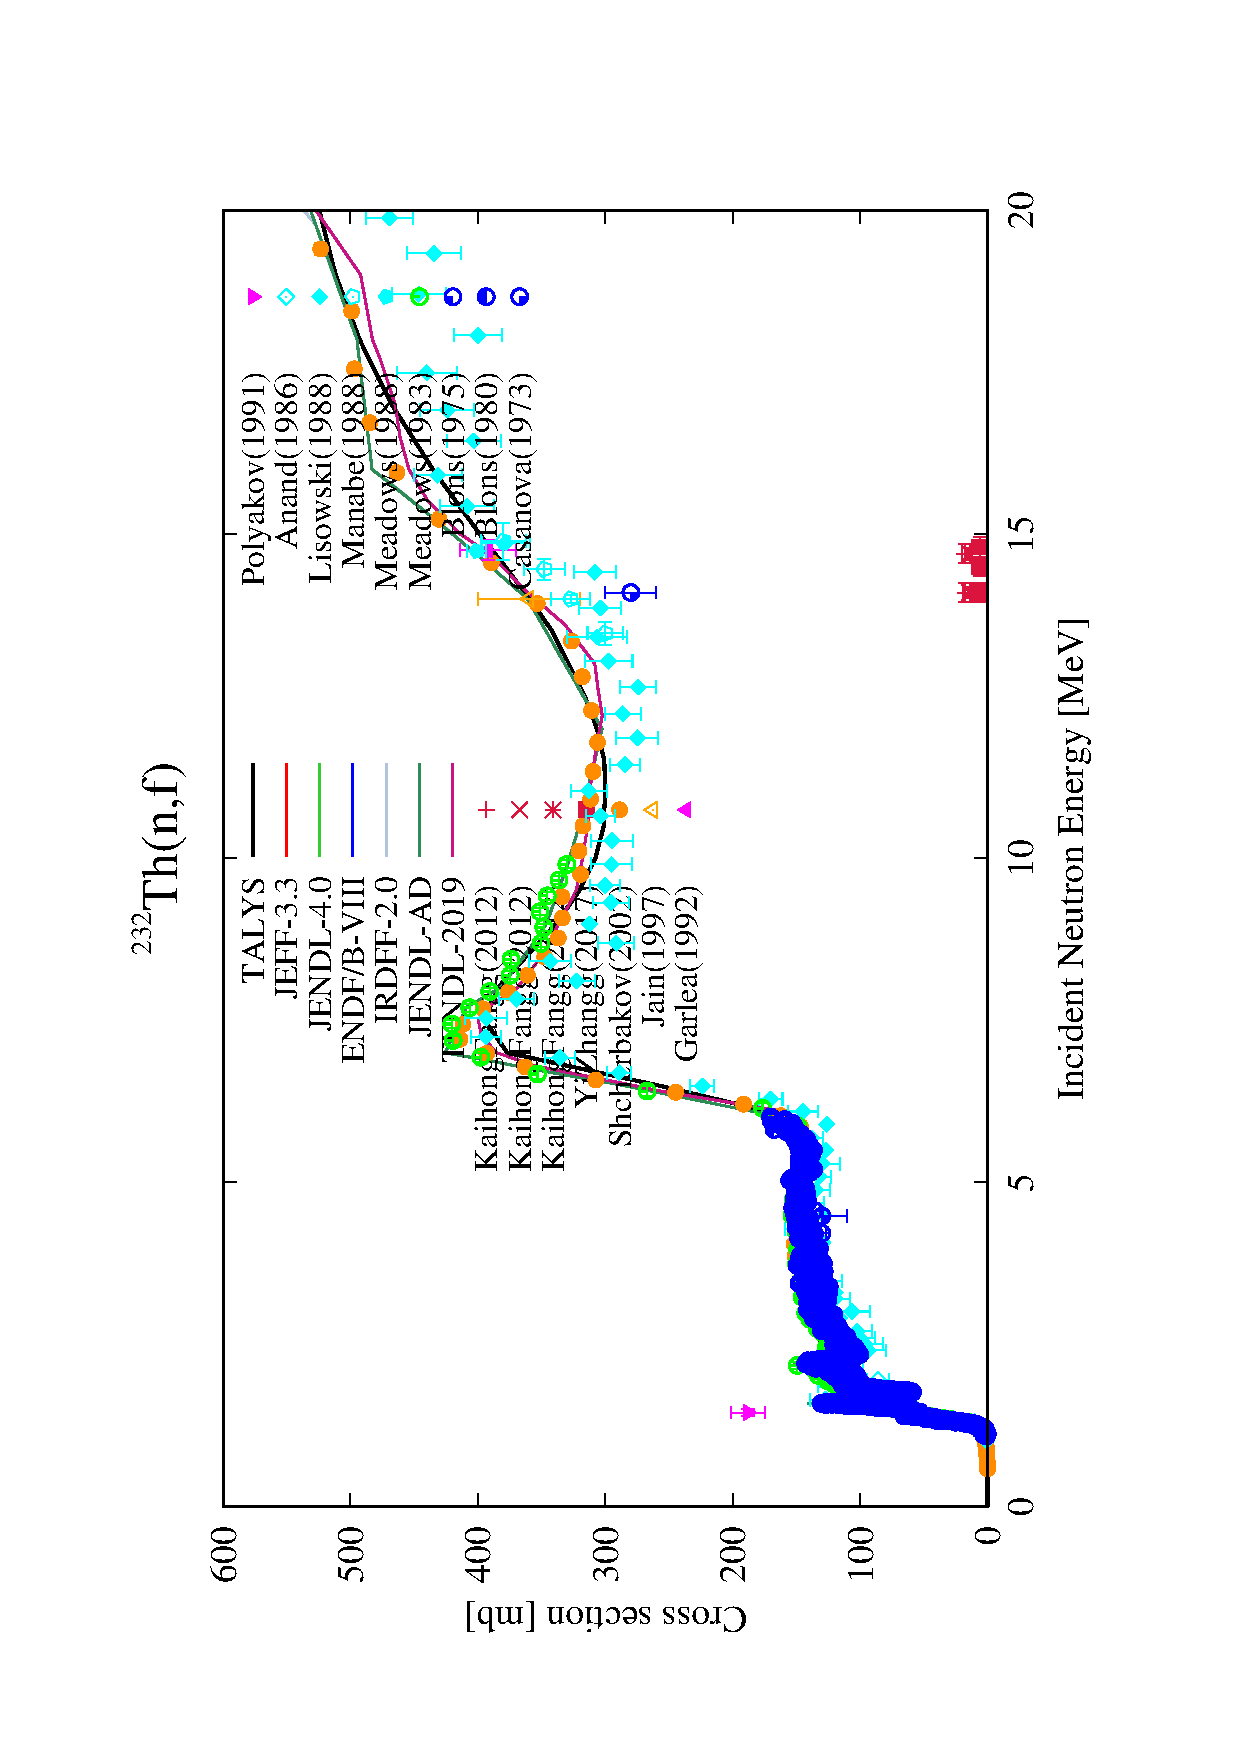
\includegraphics[scale=0.5,angle=270]{n-Th232-fis-wkb}
\caption{Neutron induced fission cross section of ${}^{232}$Th compared with
experimental data.}
\label{fissioneps}
\end{figure}
